% System overview of the v0 pilot (Figure 1 of the v0 paper). TikZ source; compile with pdflatex.
\documentclass[tikz,border=3pt]{standalone}
\usepackage[T1]{fontenc}
\usepackage[scaled=0.92]{helvet}
\renewcommand{\familydefault}{\sfdefault}
\usetikzlibrary{arrows.meta,backgrounds,calc,shapes.misc}
\definecolor{inpfill}{HTML}{F2F2F2}\definecolor{inpline}{HTML}{4D4D4D}
\definecolor{aifill}{HTML}{DCEEFB}\definecolor{ailine}{HTML}{0072B2}
\definecolor{orfill}{HTML}{E3F4EC}\definecolor{orline}{HTML}{009E73}
\definecolor{badfill}{HTML}{FBE3D6}\definecolor{badline}{HTML}{D55E00}
\definecolor{outfill}{HTML}{FFF2CC}\definecolor{outline}{HTML}{B07D00}
\definecolor{zone}{HTML}{9A9A9A}
\hyphenpenalty=10000\exhyphenpenalty=10000
\begin{document}
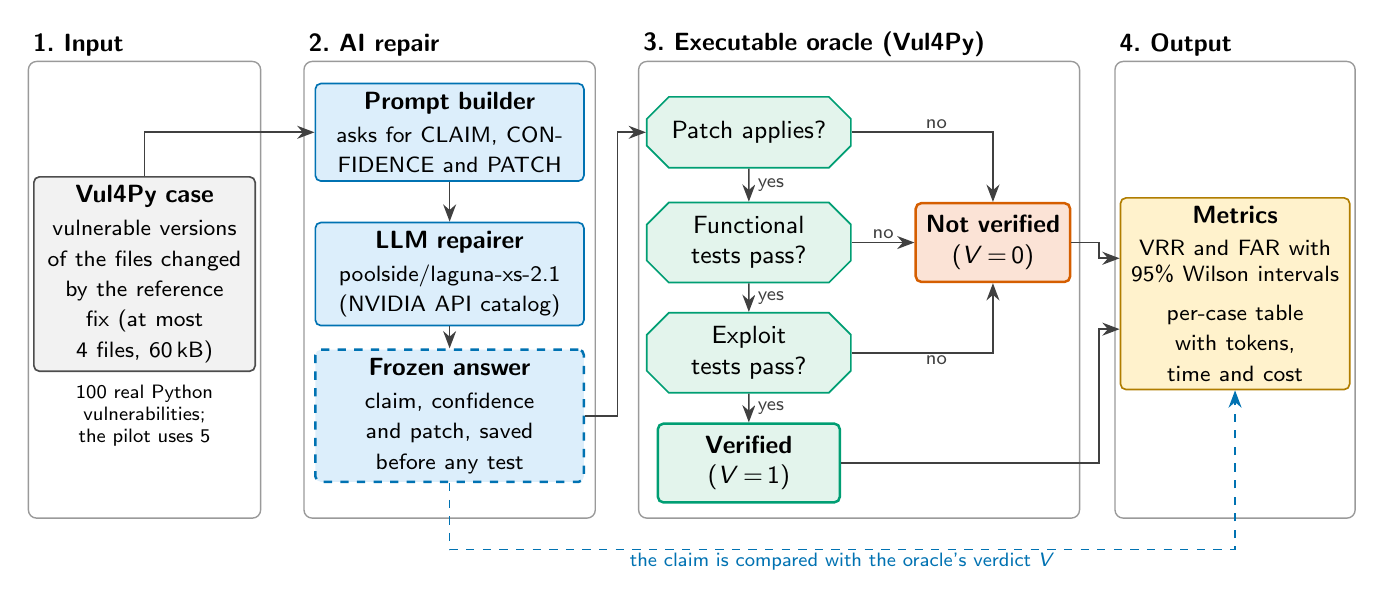
\begin{tikzpicture}[
  font=\small,
  box/.style={draw, rounded corners=2pt, align=center, text width=#1, minimum height=1.0cm, inner sep=3pt, line width=0.6pt},
  box/.default=2.75cm,
  check/.style={draw, chamfered rectangle, chamfered rectangle xsep=5pt, align=center, text width=2.1cm,
                minimum height=0.9cm, inner sep=2pt, line width=0.6pt, fill=orfill, draw=orline},
  arr/.style={-{Stealth[length=2.2mm]}, line width=0.6pt, color=black!75},
  lab/.style={font=\scriptsize, fill=white, inner sep=1pt},
  zonetitle/.style={font=\small\bfseries, anchor=south west, inner sep=1.5pt}
]
% ---------------------------------------------------------------- zones (same height)
\def\ztop{0.75}\def\zbot{-5.05}
\foreach \xa/\xb/\t in {0.0/2.95/{1.\ Input}, 3.5/7.2/{2.\ AI repair}, 7.75/13.35/{3.\ Executable oracle (Vul4Py)}, 13.8/16.85/{4.\ Output}}{
  \draw[zone, rounded corners=3pt, line width=0.5pt] (\xa,\zbot) rectangle (\xb,\ztop);
  \node[zonetitle] at (\xa,\ztop) {\t};
}
% ---------------------------------------------------------------- nodes
\node[box=2.6cm, fill=inpfill, draw=inpline] (case) at (1.475,-1.95)
  {\textbf{Vul4Py case}\\[1pt]\footnotesize vulnerable versions of the files changed by the reference fix (at most 4 files, 60\,kB)};
\node[font=\scriptsize, align=center, text width=2.6cm] at (1.475,-3.75) {100 real Python vulnerabilities;\\the pilot uses 5};

\node[box=3.2cm, fill=aifill, draw=ailine] (prompt) at (5.35,-0.15)
  {\textbf{Prompt builder}\\[1pt]\footnotesize asks for CLAIM, CONFIDENCE and PATCH};
\node[box=3.2cm, fill=aifill, draw=ailine] (llm) at (5.35,-1.95)
  {\textbf{LLM repairer}\\[1pt]\footnotesize poolside/laguna-xs-2.1 (NVIDIA API catalog)};
\node[box=3.2cm, fill=aifill, draw=ailine, line width=0.9pt, dashed] (frozen) at (5.35,-3.75)
  {\textbf{Frozen answer}\\[1pt]\footnotesize claim, confidence and patch, saved before any test};

\node[check] (applies) at (9.15,-0.15) {Patch applies?};
\node[check] (func) at (9.15,-1.55) {Functional tests pass?};
\node[check] (exploit) at (9.15,-2.95) {Exploit tests pass?};
\node[box=2.1cm, fill=orfill, draw=orline, line width=0.9pt] (ver) at (9.15,-4.35) {\textbf{Verified}\\(\textit{V}\,=\,1)};
\node[box=1.75cm, fill=badfill, draw=badline, line width=0.9pt] (notver) at (12.25,-1.55) {\textbf{Not verified}\\(\textit{V}\,=\,0)};

\node[box=2.7cm, fill=outfill, draw=outline, minimum height=2.3cm] (metrics) at (15.325,-2.2)
  {\textbf{Metrics}\\[2pt]\footnotesize VRR and FAR with 95\% Wilson intervals\\[3pt]per-case table with tokens, time and cost};

% ---------------------------------------------------------------- arrows
\draw[arr] (case.north) |- (prompt.west);
\draw[arr] (prompt) -- (llm);
\draw[arr] (llm) -- (frozen);
\draw[arr] (frozen.east) -- (7.48,-3.75) |- (applies.west);
\draw[arr] (applies) -- node[lab, right=2pt] {yes} (func);
\draw[arr] (func) -- node[lab, right=2pt] {yes} (exploit);
\draw[arr] (exploit) -- node[lab, right=2pt] {yes} (ver);
\draw[arr] (applies.east) -| node[lab, pos=0.3, above] {no} (notver.north);
\draw[arr] (func.east) -- node[lab, above] {no} (notver.west);
\draw[arr] (exploit.east) -| node[lab, pos=0.3, below] {no} (notver.south);
\draw[arr] (notver.east) -- (13.6,-1.55) |- ($(metrics.west)+(0,0.45)$);
\draw[arr] (ver.east) -- (13.6,-4.35) |- ($(metrics.west)+(0,-0.45)$);
\draw[arr, dashed, color=ailine] (frozen.south) -- (5.35,-5.45) -| node[lab, pos=0.25, below, text=ailine] {the claim is compared with the oracle's verdict \textit{V}} (metrics.south);
\end{tikzpicture}
\end{document}
